


% Header, overrides base

    % Make sure that the sphinx doc style knows who it inherits from.
    \def\sphinxdocclass{article}

    % Declare the document class
    \documentclass[letterpaper,10pt,english]{/usr/share/sphinx/texinputs/sphinxhowto}

    % Imports
    \usepackage[utf8]{inputenc}
    \DeclareUnicodeCharacter{00A0}{\\nobreakspace}
    \usepackage[T1]{fontenc}
    \usepackage{babel}
    \usepackage{times}
    \usepackage{import}
    \usepackage[Bjarne]{/usr/share/sphinx/texinputs/fncychap}
    \usepackage{longtable}
    \usepackage{/usr/share/sphinx/texinputs/sphinx}
    \usepackage{multirow}

    \usepackage{amsmath}
    \usepackage{amssymb}
    \usepackage{ucs}
    \usepackage{enumerate}

    % Used to make the Input/Output rules follow around the contents.
    \usepackage{needspace}

    % Pygments requirements
    \usepackage{fancyvrb}
    \usepackage{color}
    % ansi colors additions
    \definecolor{darkgreen}{rgb}{.12,.54,.11}
    \definecolor{lightgray}{gray}{.95}
    \definecolor{brown}{rgb}{0.54,0.27,0.07}
    \definecolor{purple}{rgb}{0.5,0.0,0.5}
    \definecolor{darkgray}{gray}{0.25}
    \definecolor{lightred}{rgb}{1.0,0.39,0.28}
    \definecolor{lightgreen}{rgb}{0.48,0.99,0.0}
    \definecolor{lightblue}{rgb}{0.53,0.81,0.92}
    \definecolor{lightpurple}{rgb}{0.87,0.63,0.87}
    \definecolor{lightcyan}{rgb}{0.5,1.0,0.83}

    % Needed to box output/input
    \usepackage{tikz}
        \usetikzlibrary{calc,arrows,shadows}
    \usepackage[framemethod=tikz]{mdframed}

    \usepackage{alltt}

    % Used to load and display graphics
    \usepackage{graphicx}
    \graphicspath{ {figs/} }
    \usepackage[Export]{adjustbox} % To resize

    % used so that images for notebooks which have spaces in the name can still be included
    \usepackage{grffile}


    % For formatting output while also word wrapping.
    \usepackage{listings}
    \lstset{breaklines=true}
    \lstset{basicstyle=\small\ttfamily}
    \def\smaller{\fontsize{9.5pt}{9.5pt}\selectfont}

    %Pygments definitions
    
\makeatletter
\def\PY@reset{\let\PY@it=\relax \let\PY@bf=\relax%
    \let\PY@ul=\relax \let\PY@tc=\relax%
    \let\PY@bc=\relax \let\PY@ff=\relax}
\def\PY@tok#1{\csname PY@tok@#1\endcsname}
\def\PY@toks#1+{\ifx\relax#1\empty\else%
    \PY@tok{#1}\expandafter\PY@toks\fi}
\def\PY@do#1{\PY@bc{\PY@tc{\PY@ul{%
    \PY@it{\PY@bf{\PY@ff{#1}}}}}}}
\def\PY#1#2{\PY@reset\PY@toks#1+\relax+\PY@do{#2}}

\expandafter\def\csname PY@tok@gd\endcsname{\def\PY@tc##1{\textcolor[rgb]{0.63,0.00,0.00}{##1}}}
\expandafter\def\csname PY@tok@gu\endcsname{\let\PY@bf=\textbf\def\PY@tc##1{\textcolor[rgb]{0.50,0.00,0.50}{##1}}}
\expandafter\def\csname PY@tok@gt\endcsname{\def\PY@tc##1{\textcolor[rgb]{0.00,0.27,0.87}{##1}}}
\expandafter\def\csname PY@tok@gs\endcsname{\let\PY@bf=\textbf}
\expandafter\def\csname PY@tok@gr\endcsname{\def\PY@tc##1{\textcolor[rgb]{1.00,0.00,0.00}{##1}}}
\expandafter\def\csname PY@tok@cm\endcsname{\let\PY@it=\textit\def\PY@tc##1{\textcolor[rgb]{0.25,0.50,0.50}{##1}}}
\expandafter\def\csname PY@tok@vg\endcsname{\def\PY@tc##1{\textcolor[rgb]{0.10,0.09,0.49}{##1}}}
\expandafter\def\csname PY@tok@m\endcsname{\def\PY@tc##1{\textcolor[rgb]{0.40,0.40,0.40}{##1}}}
\expandafter\def\csname PY@tok@mh\endcsname{\def\PY@tc##1{\textcolor[rgb]{0.40,0.40,0.40}{##1}}}
\expandafter\def\csname PY@tok@go\endcsname{\def\PY@tc##1{\textcolor[rgb]{0.53,0.53,0.53}{##1}}}
\expandafter\def\csname PY@tok@ge\endcsname{\let\PY@it=\textit}
\expandafter\def\csname PY@tok@vc\endcsname{\def\PY@tc##1{\textcolor[rgb]{0.10,0.09,0.49}{##1}}}
\expandafter\def\csname PY@tok@il\endcsname{\def\PY@tc##1{\textcolor[rgb]{0.40,0.40,0.40}{##1}}}
\expandafter\def\csname PY@tok@cs\endcsname{\let\PY@it=\textit\def\PY@tc##1{\textcolor[rgb]{0.25,0.50,0.50}{##1}}}
\expandafter\def\csname PY@tok@cp\endcsname{\def\PY@tc##1{\textcolor[rgb]{0.74,0.48,0.00}{##1}}}
\expandafter\def\csname PY@tok@gi\endcsname{\def\PY@tc##1{\textcolor[rgb]{0.00,0.63,0.00}{##1}}}
\expandafter\def\csname PY@tok@gh\endcsname{\let\PY@bf=\textbf\def\PY@tc##1{\textcolor[rgb]{0.00,0.00,0.50}{##1}}}
\expandafter\def\csname PY@tok@ni\endcsname{\let\PY@bf=\textbf\def\PY@tc##1{\textcolor[rgb]{0.60,0.60,0.60}{##1}}}
\expandafter\def\csname PY@tok@nl\endcsname{\def\PY@tc##1{\textcolor[rgb]{0.63,0.63,0.00}{##1}}}
\expandafter\def\csname PY@tok@nn\endcsname{\let\PY@bf=\textbf\def\PY@tc##1{\textcolor[rgb]{0.00,0.00,1.00}{##1}}}
\expandafter\def\csname PY@tok@no\endcsname{\def\PY@tc##1{\textcolor[rgb]{0.53,0.00,0.00}{##1}}}
\expandafter\def\csname PY@tok@na\endcsname{\def\PY@tc##1{\textcolor[rgb]{0.49,0.56,0.16}{##1}}}
\expandafter\def\csname PY@tok@nb\endcsname{\def\PY@tc##1{\textcolor[rgb]{0.00,0.50,0.00}{##1}}}
\expandafter\def\csname PY@tok@nc\endcsname{\let\PY@bf=\textbf\def\PY@tc##1{\textcolor[rgb]{0.00,0.00,1.00}{##1}}}
\expandafter\def\csname PY@tok@nd\endcsname{\def\PY@tc##1{\textcolor[rgb]{0.67,0.13,1.00}{##1}}}
\expandafter\def\csname PY@tok@ne\endcsname{\let\PY@bf=\textbf\def\PY@tc##1{\textcolor[rgb]{0.82,0.25,0.23}{##1}}}
\expandafter\def\csname PY@tok@nf\endcsname{\def\PY@tc##1{\textcolor[rgb]{0.00,0.00,1.00}{##1}}}
\expandafter\def\csname PY@tok@si\endcsname{\let\PY@bf=\textbf\def\PY@tc##1{\textcolor[rgb]{0.73,0.40,0.53}{##1}}}
\expandafter\def\csname PY@tok@s2\endcsname{\def\PY@tc##1{\textcolor[rgb]{0.73,0.13,0.13}{##1}}}
\expandafter\def\csname PY@tok@vi\endcsname{\def\PY@tc##1{\textcolor[rgb]{0.10,0.09,0.49}{##1}}}
\expandafter\def\csname PY@tok@nt\endcsname{\let\PY@bf=\textbf\def\PY@tc##1{\textcolor[rgb]{0.00,0.50,0.00}{##1}}}
\expandafter\def\csname PY@tok@nv\endcsname{\def\PY@tc##1{\textcolor[rgb]{0.10,0.09,0.49}{##1}}}
\expandafter\def\csname PY@tok@s1\endcsname{\def\PY@tc##1{\textcolor[rgb]{0.73,0.13,0.13}{##1}}}
\expandafter\def\csname PY@tok@sh\endcsname{\def\PY@tc##1{\textcolor[rgb]{0.73,0.13,0.13}{##1}}}
\expandafter\def\csname PY@tok@sc\endcsname{\def\PY@tc##1{\textcolor[rgb]{0.73,0.13,0.13}{##1}}}
\expandafter\def\csname PY@tok@sx\endcsname{\def\PY@tc##1{\textcolor[rgb]{0.00,0.50,0.00}{##1}}}
\expandafter\def\csname PY@tok@bp\endcsname{\def\PY@tc##1{\textcolor[rgb]{0.00,0.50,0.00}{##1}}}
\expandafter\def\csname PY@tok@c1\endcsname{\let\PY@it=\textit\def\PY@tc##1{\textcolor[rgb]{0.25,0.50,0.50}{##1}}}
\expandafter\def\csname PY@tok@kc\endcsname{\let\PY@bf=\textbf\def\PY@tc##1{\textcolor[rgb]{0.00,0.50,0.00}{##1}}}
\expandafter\def\csname PY@tok@c\endcsname{\let\PY@it=\textit\def\PY@tc##1{\textcolor[rgb]{0.25,0.50,0.50}{##1}}}
\expandafter\def\csname PY@tok@mf\endcsname{\def\PY@tc##1{\textcolor[rgb]{0.40,0.40,0.40}{##1}}}
\expandafter\def\csname PY@tok@err\endcsname{\def\PY@bc##1{\setlength{\fboxsep}{0pt}\fcolorbox[rgb]{1.00,0.00,0.00}{1,1,1}{\strut ##1}}}
\expandafter\def\csname PY@tok@kd\endcsname{\let\PY@bf=\textbf\def\PY@tc##1{\textcolor[rgb]{0.00,0.50,0.00}{##1}}}
\expandafter\def\csname PY@tok@ss\endcsname{\def\PY@tc##1{\textcolor[rgb]{0.10,0.09,0.49}{##1}}}
\expandafter\def\csname PY@tok@sr\endcsname{\def\PY@tc##1{\textcolor[rgb]{0.73,0.40,0.53}{##1}}}
\expandafter\def\csname PY@tok@mo\endcsname{\def\PY@tc##1{\textcolor[rgb]{0.40,0.40,0.40}{##1}}}
\expandafter\def\csname PY@tok@kn\endcsname{\let\PY@bf=\textbf\def\PY@tc##1{\textcolor[rgb]{0.00,0.50,0.00}{##1}}}
\expandafter\def\csname PY@tok@mi\endcsname{\def\PY@tc##1{\textcolor[rgb]{0.40,0.40,0.40}{##1}}}
\expandafter\def\csname PY@tok@gp\endcsname{\let\PY@bf=\textbf\def\PY@tc##1{\textcolor[rgb]{0.00,0.00,0.50}{##1}}}
\expandafter\def\csname PY@tok@o\endcsname{\def\PY@tc##1{\textcolor[rgb]{0.40,0.40,0.40}{##1}}}
\expandafter\def\csname PY@tok@kr\endcsname{\let\PY@bf=\textbf\def\PY@tc##1{\textcolor[rgb]{0.00,0.50,0.00}{##1}}}
\expandafter\def\csname PY@tok@s\endcsname{\def\PY@tc##1{\textcolor[rgb]{0.73,0.13,0.13}{##1}}}
\expandafter\def\csname PY@tok@kp\endcsname{\def\PY@tc##1{\textcolor[rgb]{0.00,0.50,0.00}{##1}}}
\expandafter\def\csname PY@tok@w\endcsname{\def\PY@tc##1{\textcolor[rgb]{0.73,0.73,0.73}{##1}}}
\expandafter\def\csname PY@tok@kt\endcsname{\def\PY@tc##1{\textcolor[rgb]{0.69,0.00,0.25}{##1}}}
\expandafter\def\csname PY@tok@ow\endcsname{\let\PY@bf=\textbf\def\PY@tc##1{\textcolor[rgb]{0.67,0.13,1.00}{##1}}}
\expandafter\def\csname PY@tok@sb\endcsname{\def\PY@tc##1{\textcolor[rgb]{0.73,0.13,0.13}{##1}}}
\expandafter\def\csname PY@tok@k\endcsname{\let\PY@bf=\textbf\def\PY@tc##1{\textcolor[rgb]{0.00,0.50,0.00}{##1}}}
\expandafter\def\csname PY@tok@se\endcsname{\let\PY@bf=\textbf\def\PY@tc##1{\textcolor[rgb]{0.73,0.40,0.13}{##1}}}
\expandafter\def\csname PY@tok@sd\endcsname{\let\PY@it=\textit\def\PY@tc##1{\textcolor[rgb]{0.73,0.13,0.13}{##1}}}

\def\PYZbs{\char`\\}
\def\PYZus{\char`\_}
\def\PYZob{\char`\{}
\def\PYZcb{\char`\}}
\def\PYZca{\char`\^}
\def\PYZam{\char`\&}
\def\PYZlt{\char`\<}
\def\PYZgt{\char`\>}
\def\PYZsh{\char`\#}
\def\PYZpc{\char`\%}
\def\PYZdl{\char`\$}
\def\PYZhy{\char`\-}
\def\PYZsq{\char`\'}
\def\PYZdq{\char`\"}
\def\PYZti{\char`\~}
% for compatibility with earlier versions
\def\PYZat{@}
\def\PYZlb{[}
\def\PYZrb{]}
\makeatother


    %Set pygments styles if needed...
    
        \definecolor{nbframe-border}{rgb}{0.867,0.867,0.867}
        \definecolor{nbframe-bg}{rgb}{0.969,0.969,0.969}
        \definecolor{nbframe-in-prompt}{rgb}{0.0,0.0,0.502}
        \definecolor{nbframe-out-prompt}{rgb}{0.545,0.0,0.0}

        \newenvironment{ColorVerbatim}
        {\begin{mdframed}[%
            roundcorner=1.0pt, %
            backgroundcolor=nbframe-bg, %
            userdefinedwidth=1\linewidth, %
            leftmargin=0.1\linewidth, %
            innerleftmargin=0pt, %
            innerrightmargin=0pt, %
            linecolor=nbframe-border, %
            linewidth=1pt, %
            usetwoside=false, %
            everyline=true, %
            innerlinewidth=3pt, %
            innerlinecolor=nbframe-bg, %
            middlelinewidth=1pt, %
            middlelinecolor=nbframe-bg, %
            outerlinewidth=0.5pt, %
            outerlinecolor=nbframe-border, %
            needspace=0pt
        ]}
        {\end{mdframed}}
        
        \newenvironment{InvisibleVerbatim}
        {\begin{mdframed}[leftmargin=0.1\linewidth,innerleftmargin=3pt,innerrightmargin=3pt, userdefinedwidth=1\linewidth, linewidth=0pt, linecolor=white, usetwoside=false]}
        {\end{mdframed}}

        \renewenvironment{Verbatim}[1][\unskip]
        {\begin{alltt}\smaller}
        {\end{alltt}}
    

    % Help prevent overflowing lines due to urls and other hard-to-break 
    % entities.  This doesn't catch everything...
    \sloppy

    % Document level variables
    \title{Gilad3q}
    \date{April 7, 2015}
    \release{}
    \author{Unknown Author}
    \renewcommand{\releasename}{}

    % TODO: Add option for the user to specify a logo for his/her export.
    \newcommand{\sphinxlogo}{}

    % Make the index page of the document.
    \makeindex

    % Import sphinx document type specifics.
     


% Body

    % Start of the document
    \begin{document}

        
            \maketitle
        

        


        
        \part{Simulating Gilad-Gate with three qubits only. The far qubit is ommitted.}\section{Copying the conclusing from DecayAndCorrect:}Conclusions so far: - The population of $\left|L_3\right>$ is
$\frac{1}{2}\left(\frac{g}{\Delta}\right)^2$ - The decay rate is
$\frac{1}{2}\gamma\left(\frac{g}{\Delta}\right)^2$ - This means the
number of oscillations \textasciitilde{} $\frac{\Delta}{\gamma}$ The
reason why the population of $\left|L_3\right>$ isn't affected by
$\gamma$ is that the Rabi oscillations between L1 and L3 go like
$\frac{g^{2}}{g^{2}+\Delta^{2}}\sin^{2}\left(\frac{\sqrt{g^{2}+\Delta^{2}}}{2}t\right)\sim\frac{g^{2}}{\Delta^{2}}\sin^{2}\left(\frac{\Delta}{2}t\right)$
which is a faster pace than $\gamma$.\section{Extra conclusions:}\begin{itemize}
\item
  The $\frac{1}{2}\gamma\left(\frac{g}{\Delta}\right)^2$ decay is caused
  by the amplitude of $\left|L_3\right>$ being added after correction to
  that of $\left|L_1\right>$.
\item
  Another source of decay is the double error, which has an effective
  decay rate of $\gamma_{eff}=\gamma\frac{\gamma}{\Gamma_{ec}+\gamma}$
\item
  To get oscillations we need to have a higher driving rate than both
  decay rates:

  \begin{itemize}
  \item
    $\frac{g^2}{\Delta}\gg\frac{1}{2}\gamma\left(\frac{g}{\Delta}\right)^2$
  \item
    $\frac{g^2}{\Delta}\gg\gamma\frac{\gamma}{\Gamma_{ec}+\gamma}$
  \end{itemize}
\item
  If both conditions apply, we should see $~\frac{\Delta}{\gamma}$
  oscillations.
\item
  For some reason that is as yet unclear to me, the last condition can
  be relaxed if the state $\left|111+001\right>$ has the same energy as
  L3, and the driving is
  \textbar{}L1\textgreater{}\textless{}L3\textbar{} + h.c. However if
  the driving is $\sigma_z$ and $\sigma_x$ this would ruin the Raman
  transitions.
\item
  Right now it is left to discover the reason, and to check the validity
  of the conditions above.
\end{itemize}\section{Conclusions about no-driving or pre-driving:}\begin{itemize}
\itemsep1pt\parskip0pt\parsep0pt
\item
  Before starting the process, we get a fast decay of the time order of
  $1/\gamma$, to a mixed state implied by the rate equation:
\end{itemize}

$\dot{P_{1}}  =  -\gamma P_{1}+\Gamma P_{e}\rightarrow P_{e}=\frac{\gamma}{\Gamma}P_{1}$

\begin{itemize}
\itemsep1pt\parskip0pt\parsep0pt
\item
  After a longer time, at the rate of $\frac{\gamma^2}{\Gamma}$ we get
  the rate equations with decay from the error levels:
\end{itemize}

$\begin{eqnarray*} \dot{P_{1}} & = & -2\gamma P_{1}+\Gamma P_{e}+\gamma P_{e}\\ \dot{P_{3}} & = & -2\gamma P_{3}+\gamma P_{e}\\ \dot{P_{e}} & = & 2\gamma\left(P_{1}+P_{3}\right)-\left(\Gamma+2\gamma\right)P_{e} \end{eqnarray*}$

\begin{itemize}
\itemsep1pt\parskip0pt\parsep0pt
\item
  For $\Gamma=0$ this implies 25\% population in L1, 25\% in L3 and 50\%
  in the error states.
\item
  Otherwise we get $2P_3=P_e=\frac{2\gamma}{\gamma+\Gamma}P_1$ (got it
  wrong by a factor of 2 somewhere)
\end{itemize}

    % Make sure that atleast 4 lines are below the HR
    \needspace{4\baselineskip}

    
        \vspace{6pt}
        \makebox[0.1\linewidth]{\smaller\hfill\tt\color{nbframe-in-prompt}In\hspace{4pt}{[}99{]}:\hspace{4pt}}\\*
        \vspace{-2.65\baselineskip}
        \begin{ColorVerbatim}
            \vspace{-0.7\baselineskip}
            \begin{Verbatim}[commandchars=\\\{\}]
\PY{o}{\PYZpc{}}\PY{k}{run} \PY{o}{\PYZhy{}}\PY{n}{i} \PY{l+s}{\PYZsq{}}\PY{l+s}{\PYZti{}/Dropbox/Alex/pynote/GiladGate3q.py}\PY{l+s}{\PYZsq{}}
\end{Verbatim}

            
                \vspace{-0.2\baselineskip}
            
        \end{ColorVerbatim}
    


    % Make sure that atleast 4 lines are below the HR
    \needspace{4\baselineskip}

    
        \vspace{6pt}
        \makebox[0.1\linewidth]{\smaller\hfill\tt\color{nbframe-in-prompt}In\hspace{4pt}{[}6{]}:\hspace{4pt}}\\*
        \vspace{-2.65\baselineskip}
        \begin{ColorVerbatim}
            \vspace{-0.7\baselineskip}
            \begin{Verbatim}[commandchars=\\\{\}]
\PY{n}{out} \PY{o}{=} \PY{n+nb}{dict}\PY{p}{(}\PY{p}{)}
\end{Verbatim}

            
                \vspace{-0.2\baselineskip}
            
        \end{ColorVerbatim}
    
In this simple example $\frac{g^2}{\Delta}=0.01$ which is bigger than
$\gamma\left(\frac{g}{\Delta}\right)^2=0.001$ and
$\gamma\frac{\gamma}{\Gamma_{ec}+\gamma}=0.001$. We indeed see about 10
oscillations $\frac{\Delta}{\gamma}$. However, the period is not exactly
$\frac{g^2}{4\Delta}$, and the decay rate is
$2\gamma\left(\frac{g}{\Delta}\right)^2$

    % Make sure that atleast 4 lines are below the HR
    \needspace{4\baselineskip}

    
        \vspace{6pt}
        \makebox[0.1\linewidth]{\smaller\hfill\tt\color{nbframe-in-prompt}In\hspace{4pt}{[}85{]}:\hspace{4pt}}\\*
        \vspace{-2.65\baselineskip}
        \begin{ColorVerbatim}
            \vspace{-0.7\baselineskip}
            \begin{Verbatim}[commandchars=\\\{\}]
\PY{c}{\PYZsh{} Driving is done with sigma\PYZus{}x and sigma\PYZus{}z. |11+00\PYZgt{}|1\PYZgt{} is thrown out of energy.}
\PY{k}{class} \PY{n+nc}{paramsDriveOuterLevel}\PY{p}{(}\PY{n}{paramsSigma}\PY{p}{)}\PY{p}{:}
    \PY{k}{def} \PY{n+nf}{H0}\PY{p}{(}\PY{n+nb+bp}{self}\PY{p}{)}\PY{p}{:}
        \PY{k}{return} \PY{o}{\PYZhy{}}\PY{n+nb+bp}{self}\PY{o}{.}\PY{n}{delta}\PY{o}{*}\PY{p}{(}\PY{n}{ketbra}\PY{p}{(}\PY{n}{L1}\PY{p}{)}\PY{o}{+}\PY{n}{ketbra}\PY{p}{(}\PY{n}{L2}\PY{p}{)}\PY{p}{)} \PY{o}{+} \PY{l+m+mi}{5}\PY{o}{*}\PY{n+nb+bp}{self}\PY{o}{.}\PY{n}{delta}\PY{o}{*}\PY{n}{ketbra}\PY{p}{(}\PY{p}{(}\PY{n}{ket}\PY{p}{(}\PY{l+s}{\PYZsq{}}\PY{l+s}{111}\PY{l+s}{\PYZsq{}}\PY{p}{)}\PY{o}{+}\PY{n}{ket}\PY{p}{(}\PY{l+s}{\PYZsq{}}\PY{l+s}{001}\PY{l+s}{\PYZsq{}}\PY{p}{)}\PY{p}{)}\PY{o}{.}\PY{n}{unit}\PY{p}{(}\PY{p}{)}\PY{p}{)}

\PY{n}{d} \PY{o}{=} \PY{n}{paramsDriveOuterLevel}\PY{p}{(}\PY{p}{)}
\PY{n}{d}\PY{o}{.}\PY{n}{g} \PY{o}{=} \PY{l+m+mf}{0.1}
\PY{n}{d}\PY{o}{.}\PY{n}{gamma} \PY{o}{=} \PY{l+m+mf}{0.1}
\PY{n}{d}\PY{o}{.}\PY{n}{delta} \PY{o}{=} \PY{l+m+mi}{1}
\PY{n}{d}\PY{o}{.}\PY{n}{gec} \PY{o}{=} \PY{l+m+mi}{10}

\PY{n}{out}\PY{p}{[}\PY{n+nb}{len}\PY{p}{(}\PY{n}{In}\PY{p}{)}\PY{o}{\PYZhy{}}\PY{l+m+mi}{1}\PY{p}{]} \PY{o}{=} \PY{n}{exper}\PY{p}{(}\PY{n}{data}\PY{o}{=}\PY{n}{d}\PY{p}{)}
\PY{n}{a} \PY{o}{=} \PY{n}{out}\PY{p}{[}\PY{n+nb}{len}\PY{p}{(}\PY{n}{In}\PY{p}{)}\PY{o}{\PYZhy{}}\PY{l+m+mi}{1}\PY{p}{]}
\PY{n}{dc} \PY{o}{=} \PY{n}{showdecay}\PY{p}{(}\PY{n}{a}\PY{p}{)}
\PY{n}{a}\PY{o}{.}\PY{n}{pop}\PY{p}{(}\PY{p}{)}
\PY{n}{show}\PY{p}{(}\PY{p}{)}
\PY{n}{pr} \PY{o}{=} \PY{n}{showperiod}\PY{p}{(}\PY{n}{a}\PY{p}{)}
\end{Verbatim}

            
                \vspace{-0.2\baselineskip}
            
        \end{ColorVerbatim}
    

    

        % If the first block is an image, minipage the image.  Else
        % request a certain amount of space for the input text.
        \needspace{4\baselineskip}
        
        

            % Add document contents.
            
                \begin{InvisibleVerbatim}
                \vspace{-0.5\baselineskip}
\begin{alltt}decayrate:  0.00219398249229  vs gamma*(g/delta)\^{}2:  0.001
\end{alltt}

            \end{InvisibleVerbatim}
            
                \begin{InvisibleVerbatim}
                \vspace{-0.5\baselineskip}
    \begin{center}
    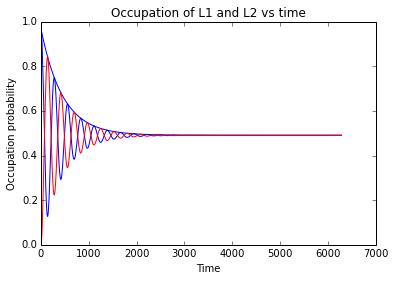
\includegraphics[max size={\textwidth}{\textheight}]{Gilad3q_files/Gilad3q_10_1.png}
    \par
    \end{center}
    
            \end{InvisibleVerbatim}
            
                \begin{InvisibleVerbatim}
                \vspace{-0.5\baselineskip}
\begin{alltt}period:  0.00360007040958  vs g\^{}2/(4*delta):  0.0025
\end{alltt}

            \end{InvisibleVerbatim}
            
                \begin{InvisibleVerbatim}
                \vspace{-0.5\baselineskip}
    \begin{center}
    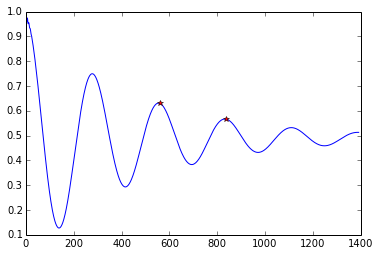
\includegraphics[max size={\textwidth}{\textheight}]{Gilad3q_files/Gilad3q_10_3.png}
    \par
    \end{center}
    
            \end{InvisibleVerbatim}
            
        
    
Doing it again with a lower $\gamma$, the decay rate is more similar to
what's expected, but the period remains off by 50\%:

    % Make sure that atleast 4 lines are below the HR
    \needspace{4\baselineskip}

    
        \vspace{6pt}
        \makebox[0.1\linewidth]{\smaller\hfill\tt\color{nbframe-in-prompt}In\hspace{4pt}{[}91{]}:\hspace{4pt}}\\*
        \vspace{-2.65\baselineskip}
        \begin{ColorVerbatim}
            \vspace{-0.7\baselineskip}
            \begin{Verbatim}[commandchars=\\\{\}]
\PY{n}{d} \PY{o}{=} \PY{n}{paramsAllOut}\PY{p}{(}\PY{p}{)}
\PY{n}{d}\PY{o}{.}\PY{n}{g} \PY{o}{=} \PY{l+m+mf}{0.1}
\PY{n}{d}\PY{o}{.}\PY{n}{gamma} \PY{o}{=} \PY{l+m+mf}{0.01}
\PY{n}{d}\PY{o}{.}\PY{n}{delta} \PY{o}{=} \PY{l+m+mi}{1}
\PY{n}{d}\PY{o}{.}\PY{n}{gec} \PY{o}{=} \PY{l+m+mi}{10}

\PY{n}{out}\PY{p}{[}\PY{n+nb}{len}\PY{p}{(}\PY{n}{In}\PY{p}{)}\PY{o}{\PYZhy{}}\PY{l+m+mi}{1}\PY{p}{]} \PY{o}{=} \PY{n}{exper}\PY{p}{(}\PY{n}{data}\PY{o}{=}\PY{n}{d}\PY{p}{)}
\PY{n}{a} \PY{o}{=} \PY{n}{out}\PY{p}{[}\PY{n+nb}{len}\PY{p}{(}\PY{n}{In}\PY{p}{)}\PY{o}{\PYZhy{}}\PY{l+m+mi}{1}\PY{p}{]}
\PY{n}{dc} \PY{o}{=} \PY{n}{showdecay}\PY{p}{(}\PY{n}{a}\PY{p}{)}
\PY{n}{a}\PY{o}{.}\PY{n}{pop}\PY{p}{(}\PY{p}{)}
\PY{n}{show}\PY{p}{(}\PY{p}{)}
\PY{n}{pr} \PY{o}{=} \PY{n}{showperiod}\PY{p}{(}\PY{n}{a}\PY{p}{)}
\end{Verbatim}

            
                \vspace{-0.2\baselineskip}
            
        \end{ColorVerbatim}
    

    

        % If the first block is an image, minipage the image.  Else
        % request a certain amount of space for the input text.
        \needspace{4\baselineskip}
        
        

            % Add document contents.
            
                \begin{InvisibleVerbatim}
                \vspace{-0.5\baselineskip}
\begin{alltt}decayrate:  0.000161777515661  vs gamma*(g/delta)\^{}2:  0.0001
\end{alltt}

            \end{InvisibleVerbatim}
            
                \begin{InvisibleVerbatim}
                \vspace{-0.5\baselineskip}
    \begin{center}
    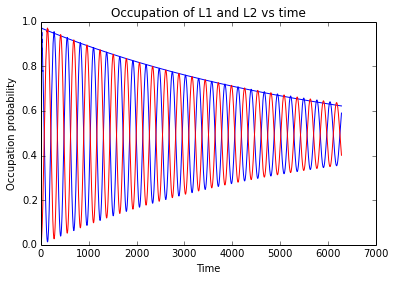
\includegraphics[max size={\textwidth}{\textheight}]{Gilad3q_files/Gilad3q_12_1.png}
    \par
    \end{center}
    
            \end{InvisibleVerbatim}
            
                \begin{InvisibleVerbatim}
                \vspace{-0.5\baselineskip}
\begin{alltt}period:  0.00364961266292  vs g\^{}2/(4*delta):  0.0025
\end{alltt}

            \end{InvisibleVerbatim}
            
                \begin{InvisibleVerbatim}
                \vspace{-0.5\baselineskip}
    \begin{center}
    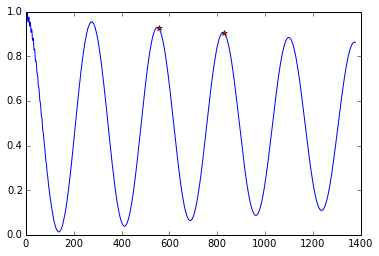
\includegraphics[max size={\textwidth}{\textheight}]{Gilad3q_files/Gilad3q_12_3.png}
    \par
    \end{center}
    
            \end{InvisibleVerbatim}
            
        
    
Now comparing the decay rate and period with the
\textbar{}L1\textgreater{}\textless{}L3\textbar{} scheme with the same
energy structure: The decay rate is different, but the period is 30
times smaller. What accounts for this change?

    % Make sure that atleast 4 lines are below the HR
    \needspace{4\baselineskip}

    
        \vspace{6pt}
        \makebox[0.1\linewidth]{\smaller\hfill\tt\color{nbframe-in-prompt}In\hspace{4pt}{[}100{]}:\hspace{4pt}}\\*
        \vspace{-2.65\baselineskip}
        \begin{ColorVerbatim}
            \vspace{-0.7\baselineskip}
            \begin{Verbatim}[commandchars=\\\{\}]
\PY{c}{\PYZsh{} Driving is done with |L1\PYZgt{}\PYZlt{}L2|. |11+00\PYZgt{}|1\PYZgt{} is thrown out of energy.}
\PY{k}{class} \PY{n+nc}{paramsOuterLevel}\PY{p}{(}\PY{n}{params}\PY{p}{)}\PY{p}{:}
    \PY{k}{def} \PY{n+nf}{H0}\PY{p}{(}\PY{n+nb+bp}{self}\PY{p}{)}\PY{p}{:}
        \PY{k}{return} \PY{o}{\PYZhy{}}\PY{n+nb+bp}{self}\PY{o}{.}\PY{n}{delta}\PY{o}{*}\PY{p}{(}\PY{n}{ketbra}\PY{p}{(}\PY{n}{L1}\PY{p}{)}\PY{o}{+}\PY{n}{ketbra}\PY{p}{(}\PY{n}{L2}\PY{p}{)}\PY{p}{)} \PY{o}{+} \PY{l+m+mi}{5}\PY{o}{*}\PY{n+nb+bp}{self}\PY{o}{.}\PY{n}{delta}\PY{o}{*}\PY{n}{ketbra}\PY{p}{(}\PY{p}{(}\PY{n}{ket}\PY{p}{(}\PY{l+s}{\PYZsq{}}\PY{l+s}{111}\PY{l+s}{\PYZsq{}}\PY{p}{)}\PY{o}{+}\PY{n}{ket}\PY{p}{(}\PY{l+s}{\PYZsq{}}\PY{l+s}{001}\PY{l+s}{\PYZsq{}}\PY{p}{)}\PY{p}{)}\PY{o}{.}\PY{n}{unit}\PY{p}{(}\PY{p}{)}\PY{p}{)}

\PY{n}{d} \PY{o}{=} \PY{n}{paramsOuterLevel}\PY{p}{(}\PY{p}{)}
\PY{n}{d}\PY{o}{.}\PY{n}{g} \PY{o}{=} \PY{l+m+mf}{0.1}
\PY{n}{d}\PY{o}{.}\PY{n}{gamma} \PY{o}{=} \PY{l+m+mf}{0.1}
\PY{n}{d}\PY{o}{.}\PY{n}{delta} \PY{o}{=} \PY{l+m+mi}{1}
\PY{n}{d}\PY{o}{.}\PY{n}{gec} \PY{o}{=} \PY{l+m+mi}{10}

\PY{n}{out}\PY{p}{[}\PY{n+nb}{len}\PY{p}{(}\PY{n}{In}\PY{p}{)}\PY{o}{\PYZhy{}}\PY{l+m+mi}{1}\PY{p}{]} \PY{o}{=} \PY{n}{exper}\PY{p}{(}\PY{n}{data}\PY{o}{=}\PY{n}{d}\PY{p}{)}
\PY{n}{a} \PY{o}{=} \PY{n}{out}\PY{p}{[}\PY{n+nb}{len}\PY{p}{(}\PY{n}{In}\PY{p}{)}\PY{o}{\PYZhy{}}\PY{l+m+mi}{1}\PY{p}{]}
\PY{n}{dc} \PY{o}{=} \PY{n}{showdecay}\PY{p}{(}\PY{n}{a}\PY{p}{)}
\PY{n}{a}\PY{o}{.}\PY{n}{pop}\PY{p}{(}\PY{p}{)}
\PY{n}{show}\PY{p}{(}\PY{p}{)}
\PY{n}{pr} \PY{o}{=} \PY{n}{showperiod}\PY{p}{(}\PY{n}{a}\PY{p}{)}
\end{Verbatim}

            
                \vspace{-0.2\baselineskip}
            
        \end{ColorVerbatim}
    

    

        % If the first block is an image, minipage the image.  Else
        % request a certain amount of space for the input text.
        \needspace{4\baselineskip}
        
        

            % Add document contents.
            
                \begin{InvisibleVerbatim}
                \vspace{-0.5\baselineskip}
\begin{alltt}decayrate:  0.000726914993065  vs gamma*(g/delta)\^{}2:  0.001
\end{alltt}

            \end{InvisibleVerbatim}
            
                \begin{InvisibleVerbatim}
                \vspace{-0.5\baselineskip}
    \begin{center}
    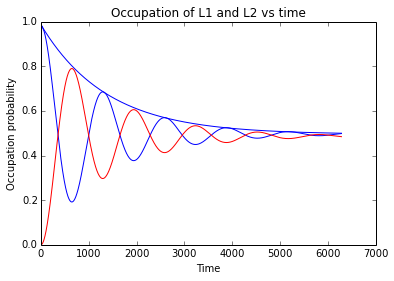
\includegraphics[max size={\textwidth}{\textheight}]{Gilad3q_files/Gilad3q_14_1.png}
    \par
    \end{center}
    
            \end{InvisibleVerbatim}
            
                \begin{InvisibleVerbatim}
                \vspace{-0.5\baselineskip}
\begin{alltt}period:  0.000773945097779  vs g\^{}2/(4*delta):  0.0025
\end{alltt}

            \end{InvisibleVerbatim}
            
                \begin{InvisibleVerbatim}
                \vspace{-0.5\baselineskip}
    \begin{center}
    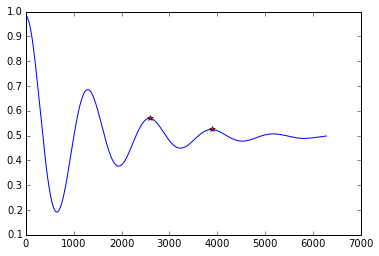
\includegraphics[max size={\textwidth}{\textheight}]{Gilad3q_files/Gilad3q_14_3.png}
    \par
    \end{center}
    
            \end{InvisibleVerbatim}
            
        
    
Just for caution we see here that the same thing happens when all other
error levels our thrown out:

    % Make sure that atleast 4 lines are below the HR
    \needspace{4\baselineskip}

    
        \vspace{6pt}
        \makebox[0.1\linewidth]{\smaller\hfill\tt\color{nbframe-in-prompt}In\hspace{4pt}{[}90{]}:\hspace{4pt}}\\*
        \vspace{-2.65\baselineskip}
        \begin{ColorVerbatim}
            \vspace{-0.7\baselineskip}
            \begin{Verbatim}[commandchars=\\\{\}]
\PY{k}{class} \PY{n+nc}{paramsAllOut}\PY{p}{(}\PY{n}{paramsSigma}\PY{p}{)}\PY{p}{:}
    \PY{k}{def} \PY{n+nf}{H0}\PY{p}{(}\PY{n+nb+bp}{self}\PY{p}{)}\PY{p}{:}
        \PY{n}{a} \PY{o}{=} \PY{l+m+mi}{5}\PY{o}{*}\PY{n+nb+bp}{self}\PY{o}{.}\PY{n}{delta}\PY{o}{*}\PY{p}{(}\PY{n}{I}\PY{o}{\PYZhy{}}\PY{n}{ketbra}\PY{p}{(}\PY{n}{ket}\PY{p}{(}\PY{l+s}{\PYZsq{}}\PY{l+s}{110}\PY{l+s}{\PYZsq{}}\PY{p}{)}\PY{p}{)}
                               \PY{o}{\PYZhy{}}\PY{n}{ketbra}\PY{p}{(}\PY{n}{ket}\PY{p}{(}\PY{l+s}{\PYZsq{}}\PY{l+s}{000}\PY{l+s}{\PYZsq{}}\PY{p}{)}\PY{p}{)}\PY{o}{\PYZhy{}}\PY{n}{ketbra}\PY{p}{(}\PY{n}{ket}\PY{p}{(}\PY{l+s}{\PYZsq{}}\PY{l+s}{111}\PY{l+s}{\PYZsq{}}\PY{p}{)}\PY{p}{)}
                               \PY{o}{\PYZhy{}}\PY{n}{ketbra}\PY{p}{(}\PY{n}{ket}\PY{p}{(}\PY{l+s}{\PYZsq{}}\PY{l+s}{001}\PY{l+s}{\PYZsq{}}\PY{p}{)}\PY{p}{)}\PY{p}{)}
        \PY{n}{a} \PY{o}{+}\PY{o}{=} \PY{o}{\PYZhy{}}\PY{n+nb+bp}{self}\PY{o}{.}\PY{n}{delta}\PY{o}{*}\PY{p}{(}\PY{n}{ketbra}\PY{p}{(}\PY{n}{L1}\PY{p}{)}\PY{o}{+}\PY{n}{ketbra}\PY{p}{(}\PY{n}{L2}\PY{p}{)}\PY{p}{)} \PY{o}{+} \PY{l+m+mi}{5}\PY{o}{*}\PY{n+nb+bp}{self}\PY{o}{.}\PY{n}{delta}\PY{o}{*}\PY{n}{ketbra}\PY{p}{(}\PY{p}{(}\PY{n}{ket}\PY{p}{(}\PY{l+s}{\PYZsq{}}\PY{l+s}{111}\PY{l+s}{\PYZsq{}}\PY{p}{)}\PY{o}{+}\PY{n}{ket}\PY{p}{(}\PY{l+s}{\PYZsq{}}\PY{l+s}{001}\PY{l+s}{\PYZsq{}}\PY{p}{)}\PY{p}{)}\PY{o}{.}\PY{n}{unit}\PY{p}{(}\PY{p}{)}\PY{p}{)}
        \PY{k}{return} \PY{n}{a}
        
\PY{n}{d} \PY{o}{=} \PY{n}{paramsAllOut}\PY{p}{(}\PY{p}{)}
\PY{n}{d}\PY{o}{.}\PY{n}{g} \PY{o}{=} \PY{l+m+mf}{0.1}
\PY{n}{d}\PY{o}{.}\PY{n}{gamma} \PY{o}{=} \PY{l+m+mf}{0.1}
\PY{n}{d}\PY{o}{.}\PY{n}{delta} \PY{o}{=} \PY{l+m+mi}{1}
\PY{n}{d}\PY{o}{.}\PY{n}{gec} \PY{o}{=} \PY{l+m+mi}{10}

\PY{n}{out}\PY{p}{[}\PY{n+nb}{len}\PY{p}{(}\PY{n}{In}\PY{p}{)}\PY{o}{\PYZhy{}}\PY{l+m+mi}{1}\PY{p}{]} \PY{o}{=} \PY{n}{exper}\PY{p}{(}\PY{n}{data}\PY{o}{=}\PY{n}{d}\PY{p}{)}
\PY{n}{a} \PY{o}{=} \PY{n}{out}\PY{p}{[}\PY{n+nb}{len}\PY{p}{(}\PY{n}{In}\PY{p}{)}\PY{o}{\PYZhy{}}\PY{l+m+mi}{1}\PY{p}{]}
\PY{n}{dc} \PY{o}{=} \PY{n}{showdecay}\PY{p}{(}\PY{n}{a}\PY{p}{)}
\PY{n}{a}\PY{o}{.}\PY{n}{pop}\PY{p}{(}\PY{p}{)}
\PY{n}{show}\PY{p}{(}\PY{p}{)}
\PY{n}{pr} \PY{o}{=} \PY{n}{showperiod}\PY{p}{(}\PY{n}{a}\PY{p}{)}
\end{Verbatim}

            
                \vspace{-0.2\baselineskip}
            
        \end{ColorVerbatim}
    

    

        % If the first block is an image, minipage the image.  Else
        % request a certain amount of space for the input text.
        \needspace{4\baselineskip}
        
        

            % Add document contents.
            
                \begin{InvisibleVerbatim}
                \vspace{-0.5\baselineskip}
\begin{alltt}decayrate:  0.00219398249229  vs gamma*(g/delta)\^{}2:  0.001
\end{alltt}

            \end{InvisibleVerbatim}
            
                \begin{InvisibleVerbatim}
                \vspace{-0.5\baselineskip}
    \begin{center}
    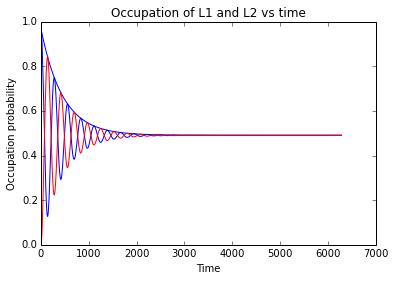
\includegraphics[max size={\textwidth}{\textheight}]{Gilad3q_files/Gilad3q_16_1.png}
    \par
    \end{center}
    
            \end{InvisibleVerbatim}
            
                \begin{InvisibleVerbatim}
                \vspace{-0.5\baselineskip}
\begin{alltt}period:  0.00360007040958  vs g\^{}2/(4*delta):  0.0025
\end{alltt}

            \end{InvisibleVerbatim}
            
                \begin{InvisibleVerbatim}
                \vspace{-0.5\baselineskip}
    \begin{center}
    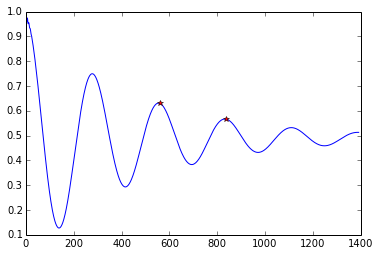
\includegraphics[max size={\textwidth}{\textheight}]{Gilad3q_files/Gilad3q_16_3.png}
    \par
    \end{center}
    
            \end{InvisibleVerbatim}
            
        
    


    % Make sure that atleast 4 lines are below the HR
    \needspace{4\baselineskip}

    
        \vspace{6pt}
        \makebox[0.1\linewidth]{\smaller\hfill\tt\color{nbframe-in-prompt}In\hspace{4pt}{[}101{]}:\hspace{4pt}}\\*
        \vspace{-2.65\baselineskip}
        \begin{ColorVerbatim}
            \vspace{-0.7\baselineskip}
            \begin{Verbatim}[commandchars=\\\{\}]
\PY{k}{class} \PY{n+nc}{paramsDriveAllOut}\PY{p}{(}\PY{n}{params}\PY{p}{)}\PY{p}{:}
    \PY{k}{def} \PY{n+nf}{H0}\PY{p}{(}\PY{n+nb+bp}{self}\PY{p}{)}\PY{p}{:}
        \PY{n}{a} \PY{o}{=} \PY{l+m+mi}{5}\PY{o}{*}\PY{n+nb+bp}{self}\PY{o}{.}\PY{n}{delta}\PY{o}{*}\PY{p}{(}\PY{n}{I}\PY{o}{\PYZhy{}}\PY{n}{ketbra}\PY{p}{(}\PY{n}{ket}\PY{p}{(}\PY{l+s}{\PYZsq{}}\PY{l+s}{110}\PY{l+s}{\PYZsq{}}\PY{p}{)}\PY{p}{)}
                               \PY{o}{\PYZhy{}}\PY{n}{ketbra}\PY{p}{(}\PY{n}{ket}\PY{p}{(}\PY{l+s}{\PYZsq{}}\PY{l+s}{000}\PY{l+s}{\PYZsq{}}\PY{p}{)}\PY{p}{)}\PY{o}{\PYZhy{}}\PY{n}{ketbra}\PY{p}{(}\PY{n}{ket}\PY{p}{(}\PY{l+s}{\PYZsq{}}\PY{l+s}{111}\PY{l+s}{\PYZsq{}}\PY{p}{)}\PY{p}{)}
                               \PY{o}{\PYZhy{}}\PY{n}{ketbra}\PY{p}{(}\PY{n}{ket}\PY{p}{(}\PY{l+s}{\PYZsq{}}\PY{l+s}{001}\PY{l+s}{\PYZsq{}}\PY{p}{)}\PY{p}{)}\PY{p}{)}
        \PY{n}{a} \PY{o}{+}\PY{o}{=} \PY{o}{\PYZhy{}}\PY{n+nb+bp}{self}\PY{o}{.}\PY{n}{delta}\PY{o}{*}\PY{p}{(}\PY{n}{ketbra}\PY{p}{(}\PY{n}{L1}\PY{p}{)}\PY{o}{+}\PY{n}{ketbra}\PY{p}{(}\PY{n}{L2}\PY{p}{)}\PY{p}{)} \PY{o}{+} \PY{l+m+mi}{5}\PY{o}{*}\PY{n+nb+bp}{self}\PY{o}{.}\PY{n}{delta}\PY{o}{*}\PY{n}{ketbra}\PY{p}{(}\PY{p}{(}\PY{n}{ket}\PY{p}{(}\PY{l+s}{\PYZsq{}}\PY{l+s}{111}\PY{l+s}{\PYZsq{}}\PY{p}{)}\PY{o}{+}\PY{n}{ket}\PY{p}{(}\PY{l+s}{\PYZsq{}}\PY{l+s}{001}\PY{l+s}{\PYZsq{}}\PY{p}{)}\PY{p}{)}\PY{o}{.}\PY{n}{unit}\PY{p}{(}\PY{p}{)}\PY{p}{)}
        \PY{k}{return} \PY{n}{a}
        
\PY{n}{d} \PY{o}{=} \PY{n}{paramsDriveAllOut}\PY{p}{(}\PY{p}{)}
\PY{n}{d}\PY{o}{.}\PY{n}{g} \PY{o}{=} \PY{l+m+mf}{0.1}
\PY{n}{d}\PY{o}{.}\PY{n}{gamma} \PY{o}{=} \PY{l+m+mf}{0.1}
\PY{n}{d}\PY{o}{.}\PY{n}{delta} \PY{o}{=} \PY{l+m+mi}{1}
\PY{n}{d}\PY{o}{.}\PY{n}{gec} \PY{o}{=} \PY{l+m+mi}{10}

\PY{n}{out}\PY{p}{[}\PY{n+nb}{len}\PY{p}{(}\PY{n}{In}\PY{p}{)}\PY{o}{\PYZhy{}}\PY{l+m+mi}{1}\PY{p}{]} \PY{o}{=} \PY{n}{exper}\PY{p}{(}\PY{n}{data}\PY{o}{=}\PY{n}{d}\PY{p}{)}
\PY{n}{a} \PY{o}{=} \PY{n}{out}\PY{p}{[}\PY{n+nb}{len}\PY{p}{(}\PY{n}{In}\PY{p}{)}\PY{o}{\PYZhy{}}\PY{l+m+mi}{1}\PY{p}{]}
\PY{n}{dc} \PY{o}{=} \PY{n}{showdecay}\PY{p}{(}\PY{n}{a}\PY{p}{)}
\PY{n}{a}\PY{o}{.}\PY{n}{pop}\PY{p}{(}\PY{p}{)}
\PY{n}{show}\PY{p}{(}\PY{p}{)}
\PY{n}{pr} \PY{o}{=} \PY{n}{showperiod}\PY{p}{(}\PY{n}{a}\PY{p}{)}
\end{Verbatim}

            
                \vspace{-0.2\baselineskip}
            
        \end{ColorVerbatim}
    

    

        % If the first block is an image, minipage the image.  Else
        % request a certain amount of space for the input text.
        \needspace{4\baselineskip}
        
        

            % Add document contents.
            
                \begin{InvisibleVerbatim}
                \vspace{-0.5\baselineskip}
\begin{alltt}decayrate:  0.000726914993065  vs gamma*(g/delta)\^{}2:  0.001
\end{alltt}

            \end{InvisibleVerbatim}
            
                \begin{InvisibleVerbatim}
                \vspace{-0.5\baselineskip}
    \begin{center}
    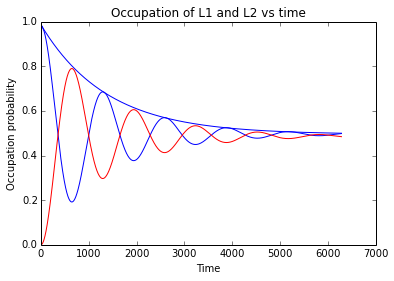
\includegraphics[max size={\textwidth}{\textheight}]{Gilad3q_files/Gilad3q_17_1.png}
    \par
    \end{center}
    
            \end{InvisibleVerbatim}
            
                \begin{InvisibleVerbatim}
                \vspace{-0.5\baselineskip}
\begin{alltt}period:  0.000773945097779  vs g\^{}2/(4*delta):  0.0025
\end{alltt}

            \end{InvisibleVerbatim}
            
                \begin{InvisibleVerbatim}
                \vspace{-0.5\baselineskip}
    \begin{center}
    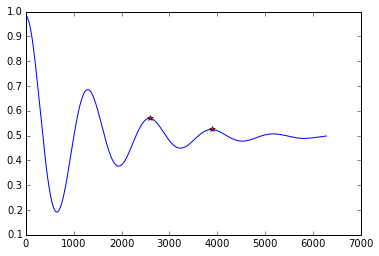
\includegraphics[max size={\textwidth}{\textheight}]{Gilad3q_files/Gilad3q_17_3.png}
    \par
    \end{center}
    
            \end{InvisibleVerbatim}
            
        
    
What happens to both systems when 111+001 remains in place? Decay rate
is reduced by a factor of \textasciitilde{}2, and the period doesn't
change for the \textbar{}L1\textgreater{}\textless{}L3\textbar{} system,
and reduces by a factor of 2 for the Sigma system.

    % Make sure that atleast 4 lines are below the HR
    \needspace{4\baselineskip}

    
        \vspace{6pt}
        \makebox[0.1\linewidth]{\smaller\hfill\tt\color{nbframe-in-prompt}In\hspace{4pt}{[}102{]}:\hspace{4pt}}\\*
        \vspace{-2.65\baselineskip}
        \begin{ColorVerbatim}
            \vspace{-0.7\baselineskip}
            \begin{Verbatim}[commandchars=\\\{\}]
\PY{n}{d1} \PY{o}{=} \PY{n}{params}\PY{p}{(}\PY{p}{)}
\PY{n}{d1}\PY{o}{.}\PY{n}{g} \PY{o}{=} \PY{l+m+mf}{0.1}
\PY{n}{d1}\PY{o}{.}\PY{n}{gamma} \PY{o}{=} \PY{l+m+mf}{0.1}
\PY{n}{d1}\PY{o}{.}\PY{n}{delta} \PY{o}{=} \PY{l+m+mi}{1}
\PY{n}{d1}\PY{o}{.}\PY{n}{gec} \PY{o}{=} \PY{l+m+mi}{10}

\PY{n}{d2} \PY{o}{=} \PY{n}{paramsSigma}\PY{p}{(}\PY{p}{)}
\PY{n}{d2}\PY{o}{.}\PY{n}{g} \PY{o}{=} \PY{l+m+mf}{0.1}
\PY{n}{d2}\PY{o}{.}\PY{n}{gamma} \PY{o}{=} \PY{l+m+mf}{0.1}
\PY{n}{d2}\PY{o}{.}\PY{n}{delta} \PY{o}{=} \PY{l+m+mi}{1}
\PY{n}{d2}\PY{o}{.}\PY{n}{gec} \PY{o}{=} \PY{l+m+mi}{10}

\PY{n}{out}\PY{p}{[}\PY{n+nb}{len}\PY{p}{(}\PY{n}{In}\PY{p}{)}\PY{o}{\PYZhy{}}\PY{l+m+mi}{1}\PY{p}{]} \PY{o}{=} \PY{n}{exper}\PY{p}{(}\PY{n}{data}\PY{o}{=}\PY{n}{d1}\PY{p}{)}
\PY{n}{a} \PY{o}{=} \PY{n}{out}\PY{p}{[}\PY{n+nb}{len}\PY{p}{(}\PY{n}{In}\PY{p}{)}\PY{o}{\PYZhy{}}\PY{l+m+mi}{1}\PY{p}{]}
\PY{n}{dc} \PY{o}{=} \PY{n}{showdecay}\PY{p}{(}\PY{n}{a}\PY{p}{)}
\PY{n}{a}\PY{o}{.}\PY{n}{pop}\PY{p}{(}\PY{p}{)}
\PY{n}{show}\PY{p}{(}\PY{p}{)}
\PY{n}{pr} \PY{o}{=} \PY{n}{showperiod}\PY{p}{(}\PY{n}{a}\PY{p}{)}
\PY{n}{show}\PY{p}{(}\PY{p}{)}

\PY{n}{out}\PY{p}{[}\PY{n+nb}{len}\PY{p}{(}\PY{n}{In}\PY{p}{)}\PY{o}{\PYZhy{}}\PY{l+m+mi}{1}\PY{p}{]} \PY{o}{=} \PY{n}{exper}\PY{p}{(}\PY{n}{data}\PY{o}{=}\PY{n}{d2}\PY{p}{)}
\PY{n}{a} \PY{o}{=} \PY{n}{out}\PY{p}{[}\PY{n+nb}{len}\PY{p}{(}\PY{n}{In}\PY{p}{)}\PY{o}{\PYZhy{}}\PY{l+m+mi}{1}\PY{p}{]}
\PY{n}{dc} \PY{o}{=} \PY{n}{showdecay}\PY{p}{(}\PY{n}{a}\PY{p}{)}
\PY{n}{a}\PY{o}{.}\PY{n}{pop}\PY{p}{(}\PY{p}{)}
\PY{n}{show}\PY{p}{(}\PY{p}{)}
\PY{n}{pr} \PY{o}{=} \PY{n}{showperiod}\PY{p}{(}\PY{n}{a}\PY{p}{)}
\end{Verbatim}

            
                \vspace{-0.2\baselineskip}
            
        \end{ColorVerbatim}
    

    

        % If the first block is an image, minipage the image.  Else
        % request a certain amount of space for the input text.
        \needspace{4\baselineskip}
        
        

            % Add document contents.
            
                \begin{InvisibleVerbatim}
                \vspace{-0.5\baselineskip}
\begin{alltt}decayrate:  0.000467198056142  vs gamma*(g/delta)\^{}2:  0.001
\end{alltt}

            \end{InvisibleVerbatim}
            
                \begin{InvisibleVerbatim}
                \vspace{-0.5\baselineskip}
    \begin{center}
    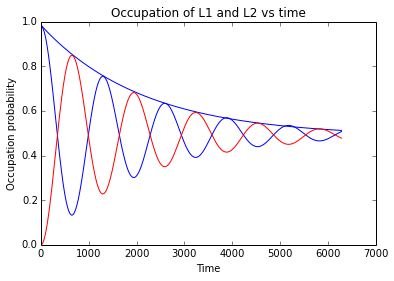
\includegraphics[max size={\textwidth}{\textheight}]{Gilad3q_files/Gilad3q_19_1.png}
    \par
    \end{center}
    
            \end{InvisibleVerbatim}
            
                \begin{InvisibleVerbatim}
                \vspace{-0.5\baselineskip}
\begin{alltt}period:  0.000773192964545  vs g\^{}2/(4*delta):  0.0025
\end{alltt}

            \end{InvisibleVerbatim}
            
                \begin{InvisibleVerbatim}
                \vspace{-0.5\baselineskip}
    \begin{center}
    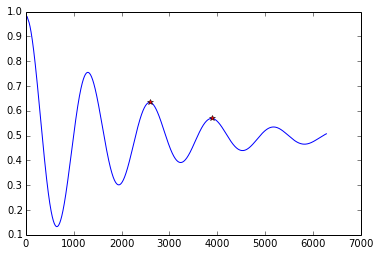
\includegraphics[max size={\textwidth}{\textheight}]{Gilad3q_files/Gilad3q_19_3.png}
    \par
    \end{center}
    
            \end{InvisibleVerbatim}
            
                \begin{InvisibleVerbatim}
                \vspace{-0.5\baselineskip}
\begin{alltt}decayrate:  0.000988986168332  vs gamma*(g/delta)\^{}2:  0.001
\end{alltt}

            \end{InvisibleVerbatim}
            
                \begin{InvisibleVerbatim}
                \vspace{-0.5\baselineskip}
    \begin{center}
    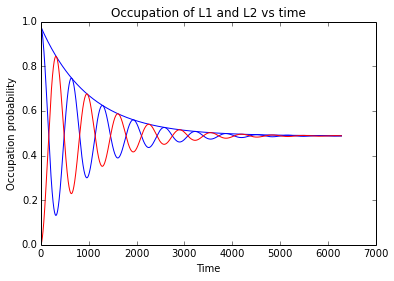
\includegraphics[max size={\textwidth}{\textheight}]{Gilad3q_files/Gilad3q_19_5.png}
    \par
    \end{center}
    
            \end{InvisibleVerbatim}
            
                \begin{InvisibleVerbatim}
                \vspace{-0.5\baselineskip}
\begin{alltt}period:  0.00154488458353  vs g\^{}2/(4*delta):  0.0025
\end{alltt}

            \end{InvisibleVerbatim}
            
                \begin{InvisibleVerbatim}
                \vspace{-0.5\baselineskip}
    \begin{center}
    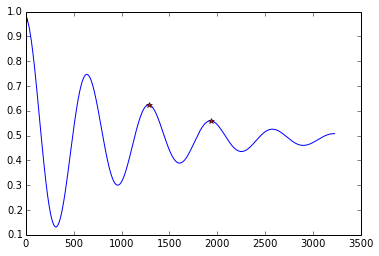
\includegraphics[max size={\textwidth}{\textheight}]{Gilad3q_files/Gilad3q_19_7.png}
    \par
    \end{center}
    
            \end{InvisibleVerbatim}
            
        
    
End of session

    % Make sure that atleast 4 lines are below the HR
    \needspace{4\baselineskip}

    
        \vspace{6pt}
        \makebox[0.1\linewidth]{\smaller\hfill\tt\color{nbframe-in-prompt}In\hspace{4pt}{[}14{]}:\hspace{4pt}}\\*
        \vspace{-2.65\baselineskip}
        \begin{ColorVerbatim}
            \vspace{-0.7\baselineskip}
            \begin{Verbatim}[commandchars=\\\{\}]
\PY{n}{d} \PY{o}{=} \PY{n}{params}\PY{p}{(}\PY{p}{)}
\PY{n}{d}\PY{o}{.}\PY{n}{g} \PY{o}{=} \PY{l+m+mf}{0.1}
\PY{n}{d}\PY{o}{.}\PY{n}{gamma} \PY{o}{=} \PY{l+m+mf}{0.1}
\PY{n}{d}\PY{o}{.}\PY{n}{delta} \PY{o}{=} \PY{l+m+mi}{1}
\PY{n}{d}\PY{o}{.}\PY{n}{gec} \PY{o}{=} \PY{l+m+mi}{10}

\PY{n}{out}\PY{p}{[}\PY{n+nb}{len}\PY{p}{(}\PY{n}{In}\PY{p}{)}\PY{o}{\PYZhy{}}\PY{l+m+mi}{1}\PY{p}{]} \PY{o}{=} \PY{n}{exper}\PY{p}{(}\PY{n}{data}\PY{o}{=}\PY{n}{d}\PY{p}{)}
\PY{n}{a} \PY{o}{=} \PY{n}{out}\PY{p}{[}\PY{n+nb}{len}\PY{p}{(}\PY{n}{In}\PY{p}{)}\PY{o}{\PYZhy{}}\PY{l+m+mi}{1}\PY{p}{]}
\PY{n}{a}\PY{o}{.}\PY{n}{pop}\PY{p}{(}\PY{p}{)}
\end{Verbatim}

            
                \vspace{-0.2\baselineskip}
            
        \end{ColorVerbatim}
    

    

        % If the first block is an image, minipage the image.  Else
        % request a certain amount of space for the input text.
        \needspace{4\baselineskip}
        
        

            % Add document contents.
            
                \begin{InvisibleVerbatim}
                \vspace{-0.5\baselineskip}
    \begin{center}
    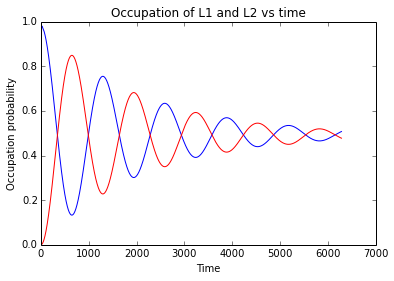
\includegraphics[max size={\textwidth}{\textheight}]{Gilad3q_files/Gilad3q_21_0.png}
    \par
    \end{center}
    
            \end{InvisibleVerbatim}
            
        
    


    % Make sure that atleast 4 lines are below the HR
    \needspace{4\baselineskip}

    
        \vspace{6pt}
        \makebox[0.1\linewidth]{\smaller\hfill\tt\color{nbframe-in-prompt}In\hspace{4pt}{[}83{]}:\hspace{4pt}}\\*
        \vspace{-2.65\baselineskip}
        \begin{ColorVerbatim}
            \vspace{-0.7\baselineskip}
            \begin{Verbatim}[commandchars=\\\{\}]
\PY{n}{a} \PY{o}{=} \PY{n}{out}\PY{p}{[}\PY{l+m+mi}{14}\PY{p}{]}
\PY{n}{dc} \PY{o}{=} \PY{n}{showdecay}\PY{p}{(}\PY{n}{a}\PY{p}{)}
\PY{n}{a}\PY{o}{.}\PY{n}{pop}\PY{p}{(}\PY{p}{)}
\PY{n}{show}\PY{p}{(}\PY{p}{)}
\PY{n}{pr} \PY{o}{=} \PY{n}{showperiod}\PY{p}{(}\PY{n}{a}\PY{p}{)}
\end{Verbatim}

            
                \vspace{-0.2\baselineskip}
            
        \end{ColorVerbatim}
    

    

        % If the first block is an image, minipage the image.  Else
        % request a certain amount of space for the input text.
        \needspace{4\baselineskip}
        
        

            % Add document contents.
            
                \begin{InvisibleVerbatim}
                \vspace{-0.5\baselineskip}
\begin{alltt}decayrate:  0.000467198056142  vs gamma*(g/delta)\^{}2:  0.001
\end{alltt}

            \end{InvisibleVerbatim}
            
                \begin{InvisibleVerbatim}
                \vspace{-0.5\baselineskip}
    \begin{center}
    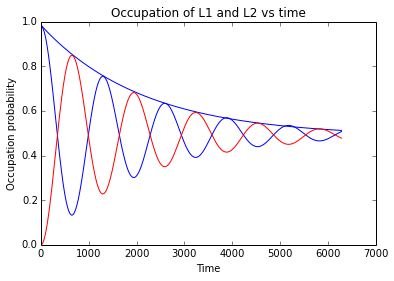
\includegraphics[max size={\textwidth}{\textheight}]{Gilad3q_files/Gilad3q_22_1.png}
    \par
    \end{center}
    
            \end{InvisibleVerbatim}
            
                \begin{InvisibleVerbatim}
                \vspace{-0.5\baselineskip}
\begin{alltt}period:  0.000773192964545  vs g\^{}2/(4*delta):  0.0025
\end{alltt}

            \end{InvisibleVerbatim}
            
                \begin{InvisibleVerbatim}
                \vspace{-0.5\baselineskip}
    \begin{center}
    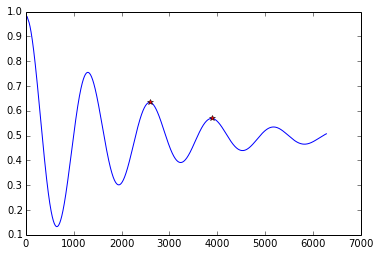
\includegraphics[max size={\textwidth}{\textheight}]{Gilad3q_files/Gilad3q_22_3.png}
    \par
    \end{center}
    
            \end{InvisibleVerbatim}
            
        
    


    % Make sure that atleast 4 lines are below the HR
    \needspace{4\baselineskip}

    
        \vspace{6pt}
        \makebox[0.1\linewidth]{\smaller\hfill\tt\color{nbframe-in-prompt}In\hspace{4pt}{[}48{]}:\hspace{4pt}}\\*
        \vspace{-2.65\baselineskip}
        \begin{ColorVerbatim}
            \vspace{-0.7\baselineskip}
            \begin{Verbatim}[commandchars=\\\{\}]
\PY{n}{d} \PY{o}{=} \PY{n}{paramsDrive}\PY{p}{(}\PY{p}{)}
\PY{n}{d}\PY{o}{.}\PY{n}{g} \PY{o}{=} \PY{l+m+mi}{1}
\PY{n}{d}\PY{o}{.}\PY{n}{gamma} \PY{o}{=} \PY{l+m+mf}{0.001}
\PY{n}{d}\PY{o}{.}\PY{n}{delta} \PY{o}{=} \PY{l+m+mi}{10}
\PY{n}{d}\PY{o}{.}\PY{n}{gec} \PY{o}{=} \PY{l+m+mi}{10}

\PY{n}{out}\PY{p}{[}\PY{n+nb}{len}\PY{p}{(}\PY{n}{In}\PY{p}{)}\PY{o}{\PYZhy{}}\PY{l+m+mi}{1}\PY{p}{]} \PY{o}{=} \PY{n}{exper}\PY{p}{(}\PY{n}{data}\PY{o}{=}\PY{n}{d}\PY{p}{)}
\PY{n}{a} \PY{o}{=} \PY{n}{out}\PY{p}{[}\PY{n+nb}{len}\PY{p}{(}\PY{n}{In}\PY{p}{)}\PY{o}{\PYZhy{}}\PY{l+m+mi}{1}\PY{p}{]}
\PY{n}{a}\PY{o}{.}\PY{n}{pop}\PY{p}{(}\PY{p}{)}
\end{Verbatim}

            
                \vspace{-0.2\baselineskip}
            
        \end{ColorVerbatim}
    

    

        % If the first block is an image, minipage the image.  Else
        % request a certain amount of space for the input text.
        \needspace{4\baselineskip}
        
        

            % Add document contents.
            
                \begin{InvisibleVerbatim}
                \vspace{-0.5\baselineskip}
    \begin{center}
    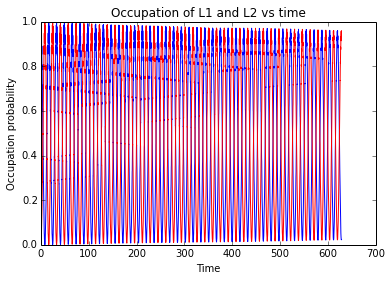
\includegraphics[max size={\textwidth}{\textheight}]{Gilad3q_files/Gilad3q_23_0.png}
    \par
    \end{center}
    
            \end{InvisibleVerbatim}
            
        
    


    % Make sure that atleast 4 lines are below the HR
    \needspace{4\baselineskip}

    
        \vspace{6pt}
        \makebox[0.1\linewidth]{\smaller\hfill\tt\color{nbframe-in-prompt}In\hspace{4pt}{[}55{]}:\hspace{4pt}}\\*
        \vspace{-2.65\baselineskip}
        \begin{ColorVerbatim}
            \vspace{-0.7\baselineskip}
            \begin{Verbatim}[commandchars=\\\{\}]
\PY{n}{a} \PY{o}{=} \PY{n}{out}\PY{p}{[}\PY{l+m+mi}{48}\PY{p}{]}
\PY{n}{vals} \PY{o}{=} \PY{n}{real}\PY{p}{(}\PY{n}{expect}\PY{p}{(}\PY{n}{ketbra}\PY{p}{(}\PY{n}{L1}\PY{p}{)}\PY{p}{,}\PY{n}{a}\PY{o}{.}\PY{n}{rho}\PY{p}{)}\PY{p}{)}
\PY{n}{smoothed} \PY{o}{=} \PY{n}{np}\PY{o}{.}\PY{n}{convolve}\PY{p}{(}\PY{n}{vals}\PY{p}{,} \PY{n}{np}\PY{o}{.}\PY{n}{ones}\PY{p}{(}\PY{l+m+mi}{10}\PY{p}{)}\PY{o}{/}\PY{l+m+mi}{10}\PY{p}{)}
\PY{n}{mini} \PY{o}{=} \PY{n}{argrelextrema}\PY{p}{(}\PY{n}{smoothed}\PY{p}{,} \PY{n}{np}\PY{o}{.}\PY{n}{less}\PY{p}{)}\PY{p}{[}\PY{l+m+mi}{0}\PY{p}{]}
\PY{n}{plot}\PY{p}{(}\PY{n}{a}\PY{o}{.}\PY{n}{timelist}\PY{p}{[}\PY{p}{:}\PY{l+m+mi}{1000}\PY{p}{]}\PY{p}{,}\PY{n}{smoothed}\PY{p}{[}\PY{p}{:}\PY{l+m+mi}{1000}\PY{p}{]}\PY{p}{)}

\PY{k}{print} \PY{n}{a}\PY{o}{.}\PY{n}{timelist}\PY{p}{[}\PY{n}{mini}\PY{p}{[}\PY{p}{:}\PY{l+m+mi}{40}\PY{p}{]}\PY{p}{]}
\PY{k}{print} \PY{n}{a}\PY{o}{.}\PY{n}{timelist}\PY{p}{[}\PY{n}{mini}\PY{p}{[}\PY{l+m+mi}{3}\PY{p}{]}\PY{p}{]}
\PY{k}{print} \PY{l+m+mi}{1}\PY{o}{/}\PY{p}{(}\PY{n}{a}\PY{o}{.}\PY{n}{timelist}\PY{p}{[}\PY{n}{mini}\PY{p}{[}\PY{l+m+mi}{1}\PY{p}{]}\PY{p}{]} \PY{o}{\PYZhy{}} \PY{n}{a}\PY{o}{.}\PY{n}{timelist}\PY{p}{[}\PY{n}{mini}\PY{p}{[}\PY{l+m+mi}{0}\PY{p}{]}\PY{p}{]}\PY{p}{)}
\end{Verbatim}

            
                \vspace{-0.2\baselineskip}
            
        \end{ColorVerbatim}
    

    

        % If the first block is an image, minipage the image.  Else
        % request a certain amount of space for the input text.
        \needspace{4\baselineskip}
        
        

            % Add document contents.
            
                \begin{InvisibleVerbatim}
                \vspace{-0.5\baselineskip}
\begin{alltt}[   8.67253023   25.01207994   41.2259408    57.56549051   73.90504022
   90.24458993  106.58413964  122.7980005   139.13755021  155.47709992
  171.81664963  179.86073564  188.15619934  196.32597419  204.49574905
  212.6655239   220.83529875  229.00507361  237.04915962  245.34462332
  253.38870933  261.68417303  269.72825904  278.02372273  286.06780874
  302.40735845  318.74690816  335.08645787  351.30031874  367.63986844
  383.97941815  400.31896786  416.53282873  432.87237843  449.21192814
  465.42578901  481.76533872  498.10488842  514.31874929  530.658299
]
57.5654905119
0.0612011969628
\end{alltt}

            \end{InvisibleVerbatim}
            
                \begin{InvisibleVerbatim}
                \vspace{-0.5\baselineskip}
    \begin{center}
    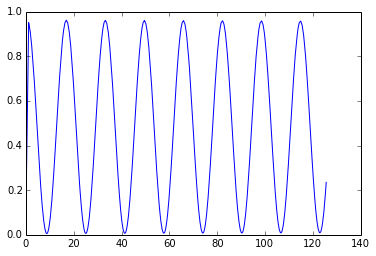
\includegraphics[max size={\textwidth}{\textheight}]{Gilad3q_files/Gilad3q_24_1.png}
    \par
    \end{center}
    
            \end{InvisibleVerbatim}
            
        
    


    % Make sure that atleast 4 lines are below the HR
    \needspace{4\baselineskip}

    
        \vspace{6pt}
        \makebox[0.1\linewidth]{\smaller\hfill\tt\color{nbframe-in-prompt}In\hspace{4pt}{[}98{]}:\hspace{4pt}}\\*
        \vspace{-2.65\baselineskip}
        \begin{ColorVerbatim}
            \vspace{-0.7\baselineskip}
            \begin{Verbatim}[commandchars=\\\{\}]
\PY{n}{L1}\PY{o}{.}\PY{n}{dag}\PY{p}{(}\PY{p}{)}\PY{o}{*}\PY{n}{tensor}\PY{p}{(}\PY{n}{sigmaz}\PY{p}{(}\PY{p}{)}\PY{p}{,}\PY{n}{qeye}\PY{p}{(}\PY{l+m+mi}{2}\PY{p}{)}\PY{p}{,}\PY{n}{qeye}\PY{p}{(}\PY{l+m+mi}{2}\PY{p}{)}\PY{p}{)}\PY{o}{*}\PY{n}{L3}
\end{Verbatim}

            
                \vspace{-0.2\baselineskip}
            
        \end{ColorVerbatim}
    

    

        % If the first block is an image, minipage the image.  Else
        % request a certain amount of space for the input text.
        \needspace{4\baselineskip}
        
        

            % Add document contents.
            
                \makebox[0.1\linewidth]{\smaller\hfill\tt\color{nbframe-out-prompt}Out\hspace{4pt}{[}98{]}:\hspace{4pt}}\\*
                \vspace{-2.55\baselineskip}\begin{InvisibleVerbatim}
                \vspace{-0.5\baselineskip}
Quantum object: dims = [[1], [1]], shape = [1, 1], type = oper, isherm = True\begin{equation*}\left(\begin{array}{*{11}c}-1.000\\\end{array}\right)\end{equation*}
            \end{InvisibleVerbatim}
            
        
    


    % Make sure that atleast 4 lines are below the HR
    \needspace{4\baselineskip}

    
        \vspace{6pt}
        \makebox[0.1\linewidth]{\smaller\hfill\tt\color{nbframe-in-prompt}In\hspace{4pt}{[}{]}:\hspace{4pt}}\\*
        \vspace{-2.65\baselineskip}
        \begin{ColorVerbatim}
            \vspace{-0.7\baselineskip}
            \begin{Verbatim}[commandchars=\\\{\}]

\end{Verbatim}

            
                \vspace{0.3\baselineskip}
            
        \end{ColorVerbatim}
    

        

        \renewcommand{\indexname}{Index}
        \printindex

    % End of document
    \end{document}


